\documentclass[notes]{beamer}
\usetheme{Rochester}

\usepackage{graphicx}

\title{Projects in Exoplanets}
\subtitle{TESS Lightcurve Photometry}
\author{Dina Sofia Mortensen \& Jesper Dam Knudgaard}
\institute{Stellar Astrophysics Centre, Aarhus University}
\date{January 18, 2019}

\begin{document}

\begin{frame}
\titlepage
\end{frame}

\section{Data Analysis}

\begin{frame}
\frametitle{Raw Data}
\centering
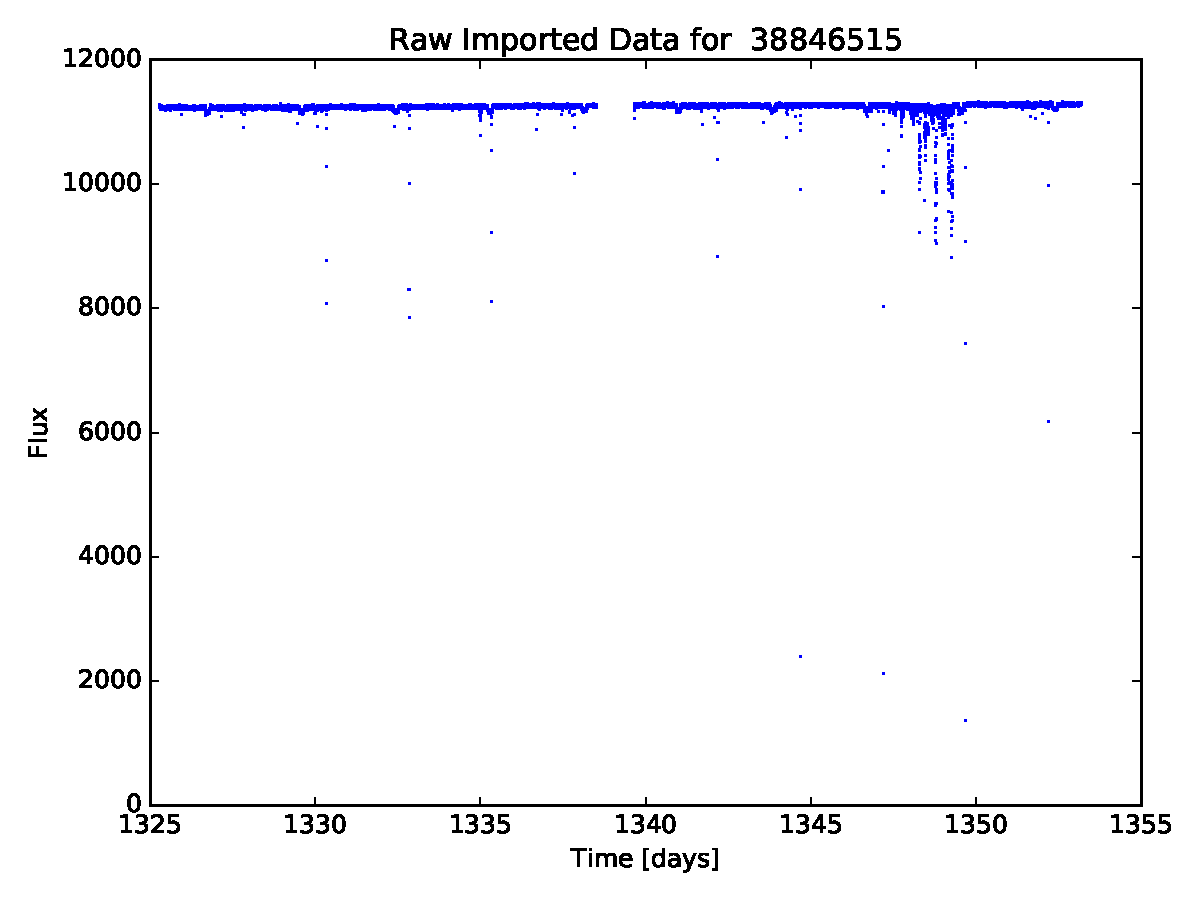
\includegraphics[width=0.9\textwidth]{../figures/2019-1-15_16:2:14_rawdata_TIC38846515.pdf}
\end{frame}

\begin{frame}
\frametitle{Normalization}
\centering
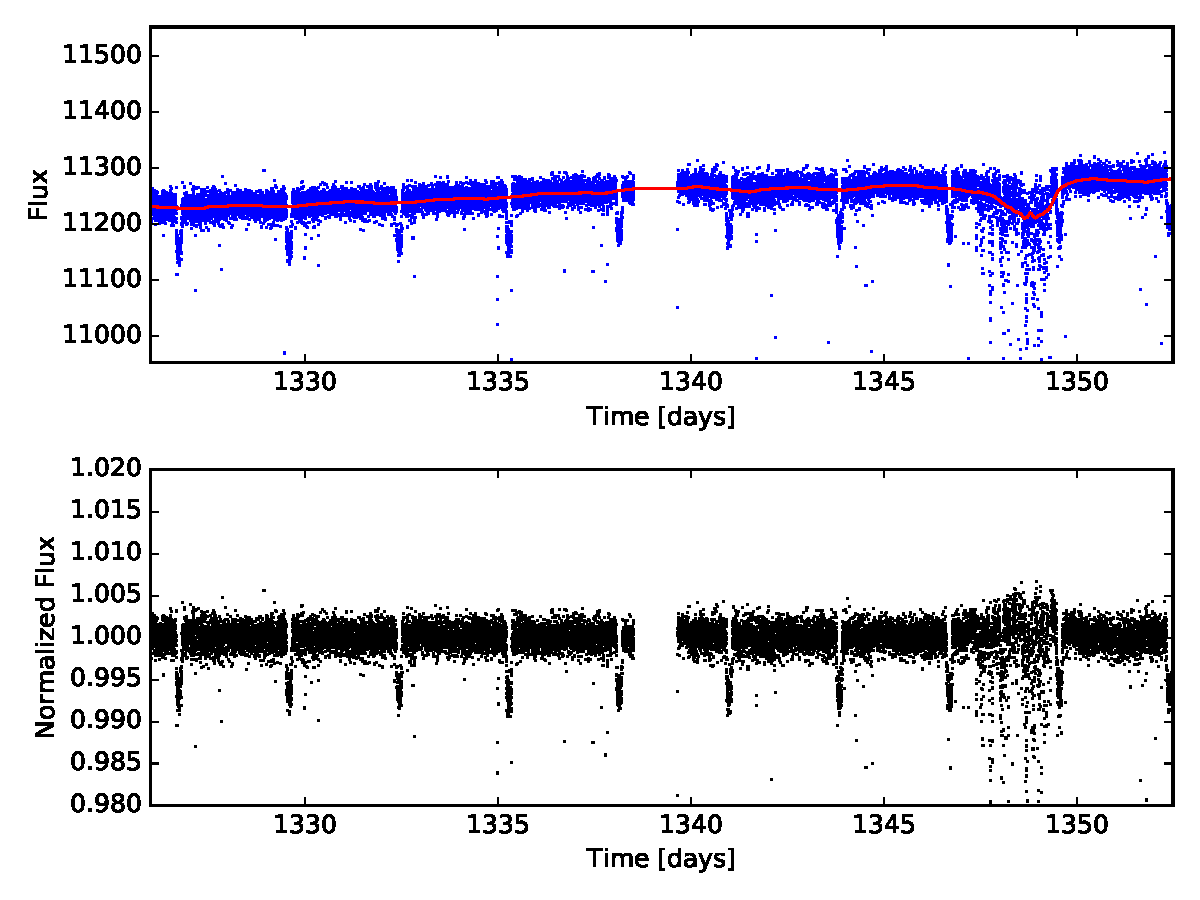
\includegraphics[width=0.9\textwidth]{../figures/2018-11-9_14:25:51_norm_curve0.pdf}
\end{frame}

\begin{frame}
\frametitle{Moving Median Filter}
\centering
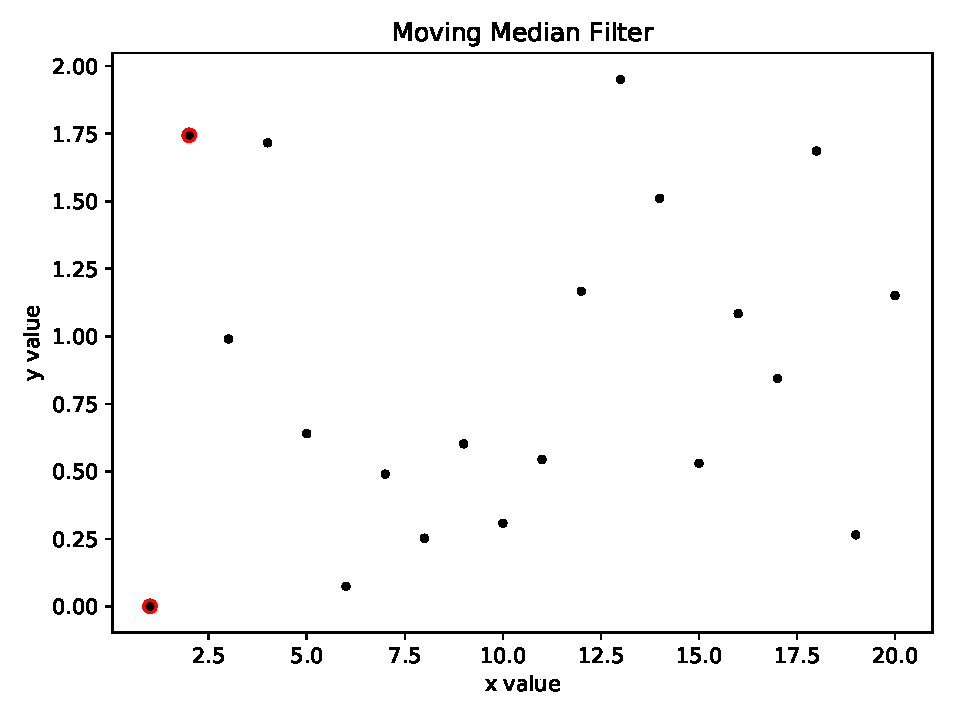
\includegraphics[width=0.9\textwidth]{../../med_filt_dem_fig/med_filt_0.pdf}
\end{frame}

\begin{frame}
\frametitle{Moving Median Filter}
\centering
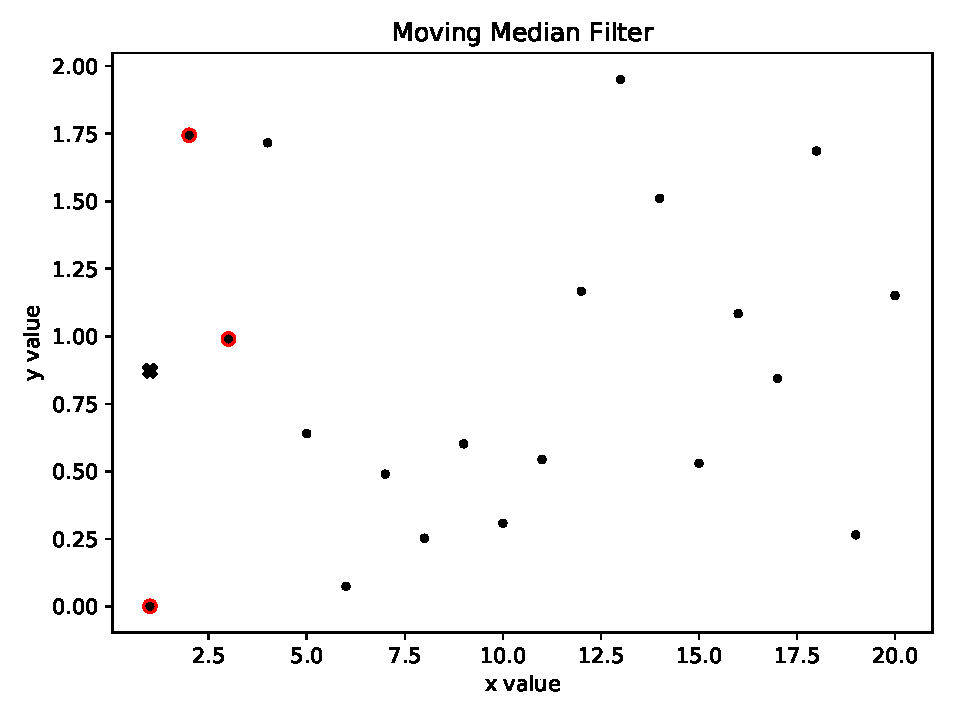
\includegraphics[width=0.9\textwidth]{../../med_filt_dem_fig/med_filt_1.pdf}
\end{frame}

\begin{frame}
\frametitle{Moving Median Filter}
\centering
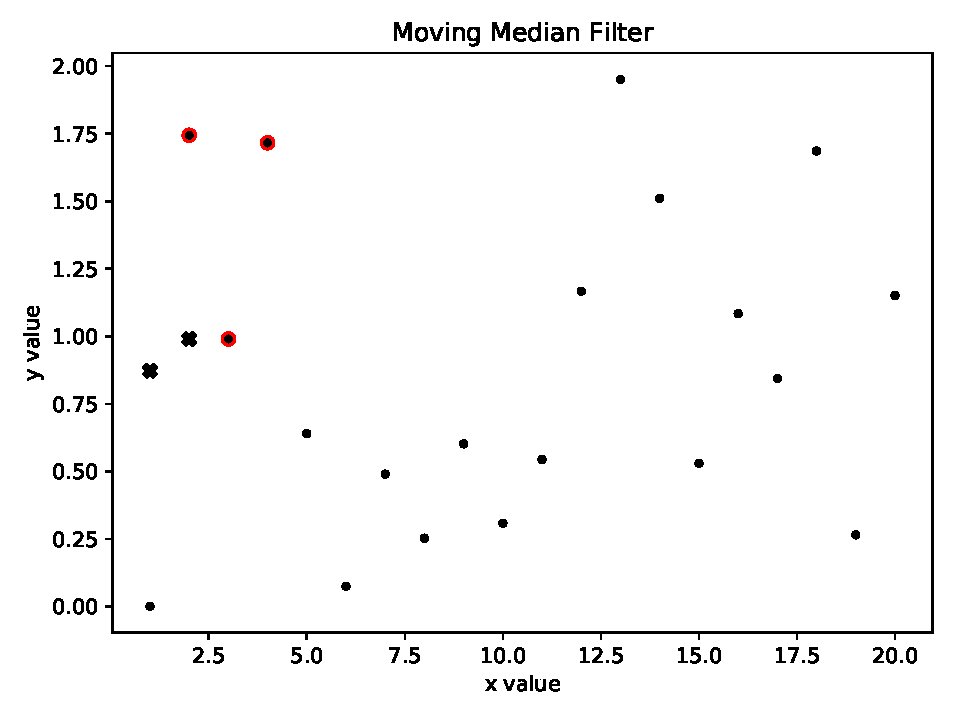
\includegraphics[width=0.9\textwidth]{../../med_filt_dem_fig/med_filt_2.pdf}
\end{frame}

\begin{frame}
\frametitle{Moving Median Filter}
\centering
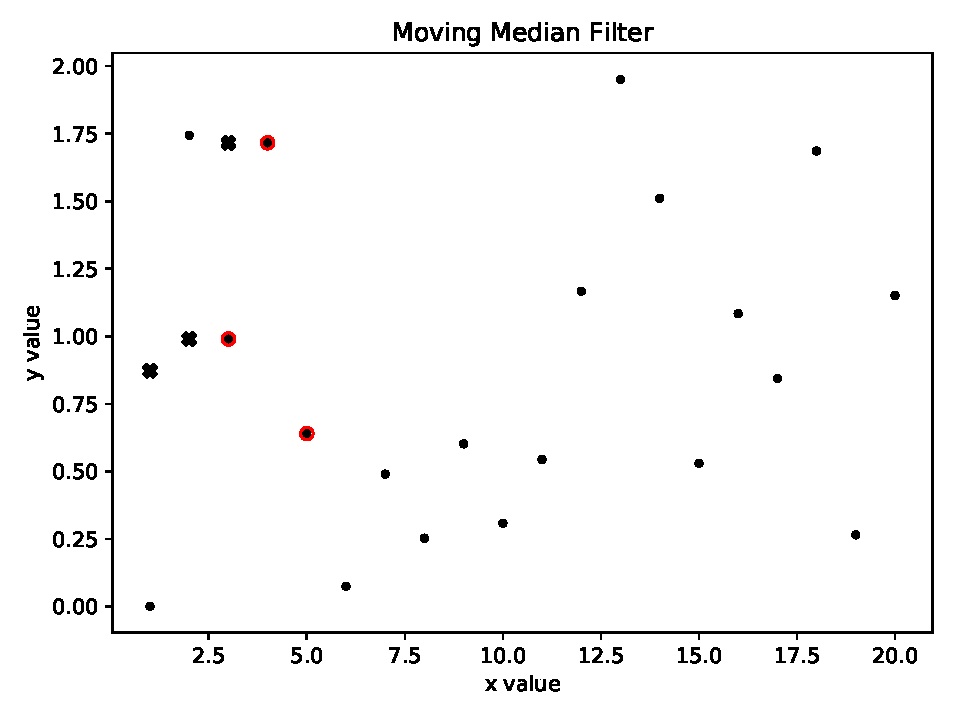
\includegraphics[width=0.9\textwidth]{../../med_filt_dem_fig/med_filt_3.pdf}
\end{frame}

\begin{frame}
\frametitle{Moving Median Filter}
\centering
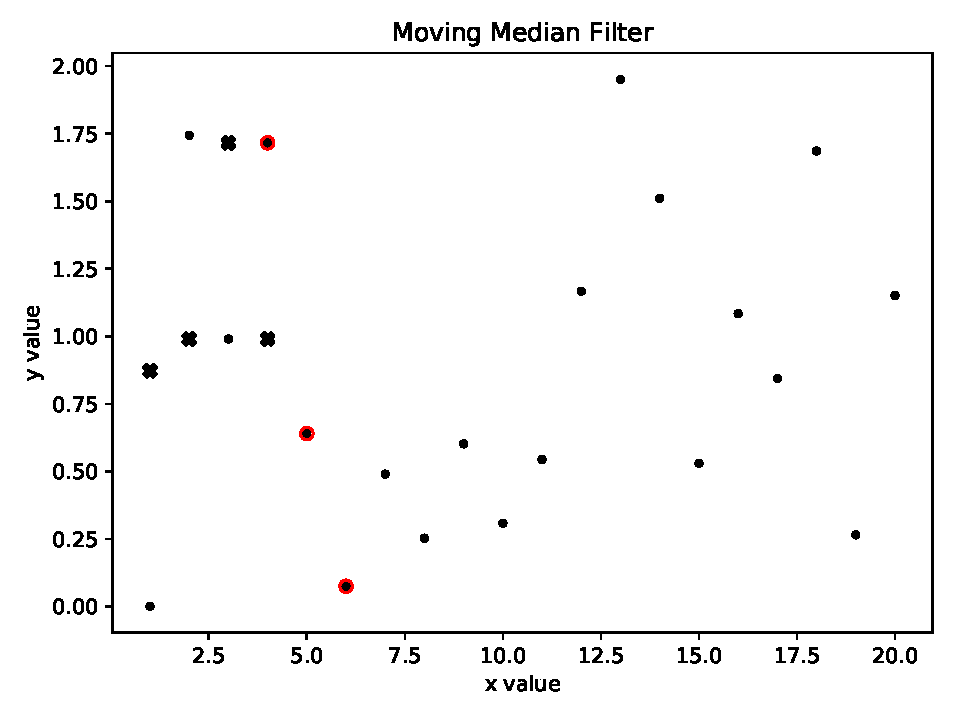
\includegraphics[width=0.9\textwidth]{../../med_filt_dem_fig/med_filt_4.pdf}
\end{frame}

\begin{frame}
\frametitle{Moving Median Filter}
\centering
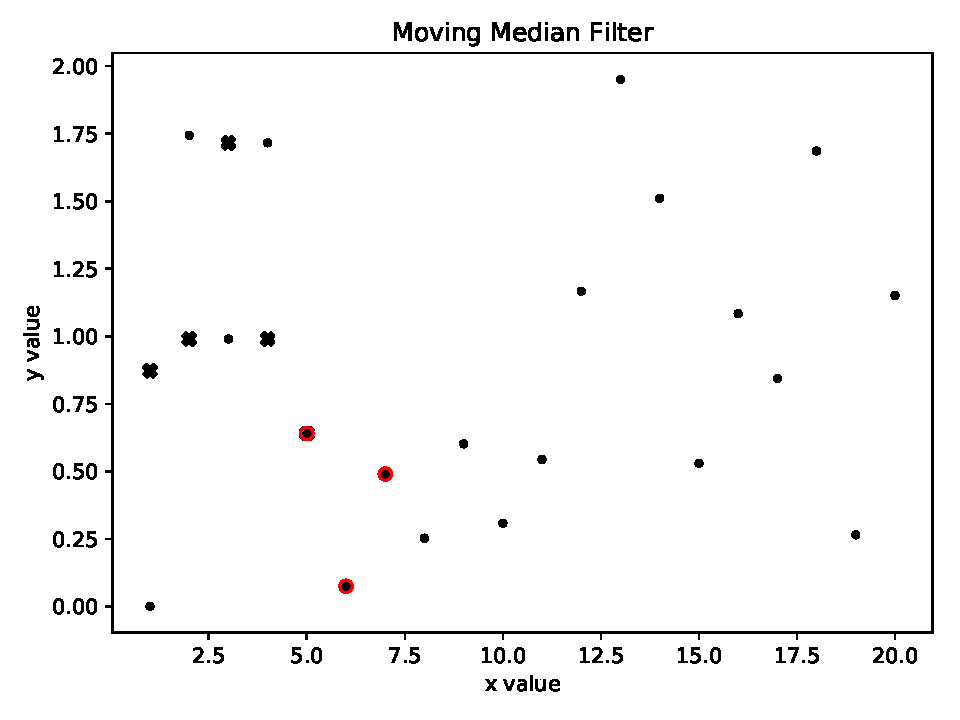
\includegraphics[width=0.9\textwidth]{../../med_filt_dem_fig/med_filt_5.pdf}
\end{frame}

\begin{frame}
\frametitle{Interpolation}
\centering
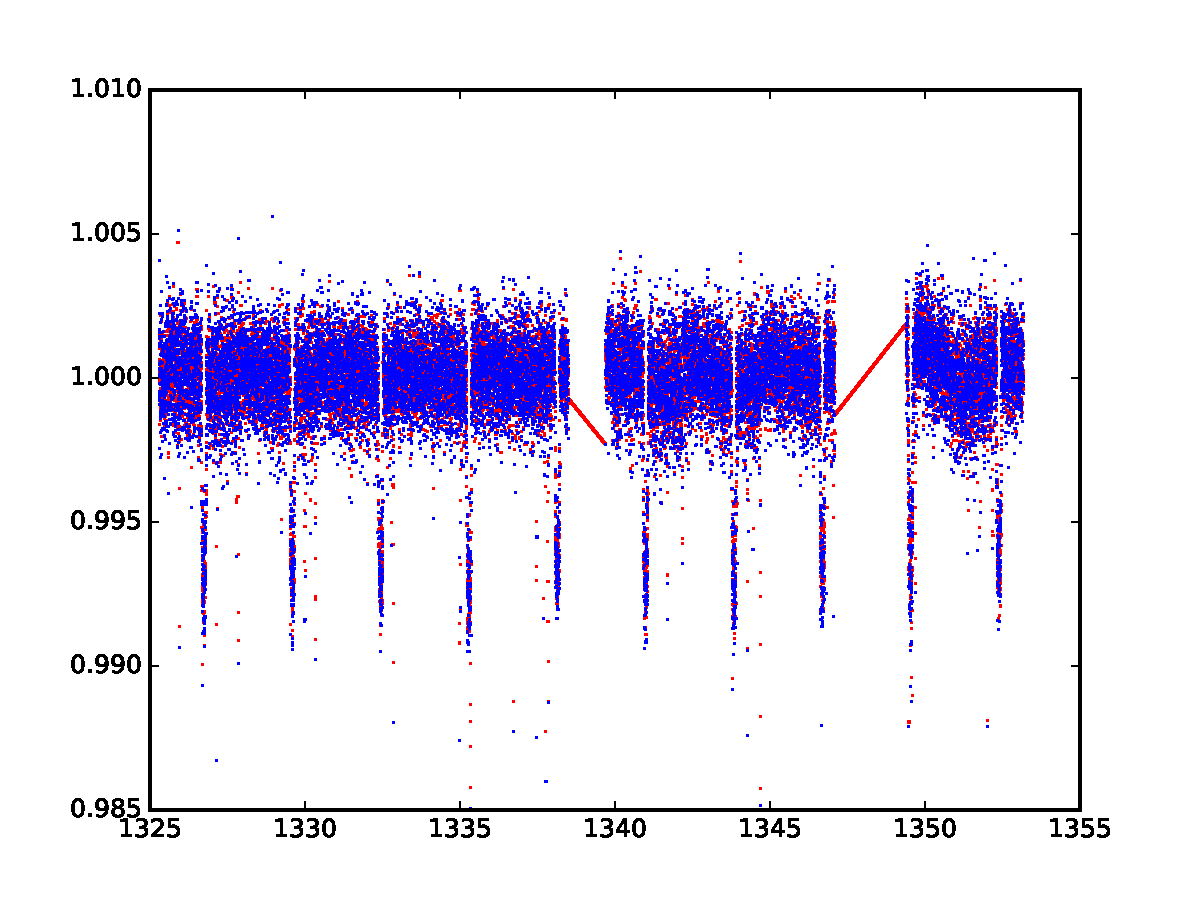
\includegraphics[width=0.9\textwidth]{../figures/2018-11-14_15:35:52_inter_curve0.pdf}
\end{frame}

\begin{frame}
\frametitle{Autocorrelation}
\centering
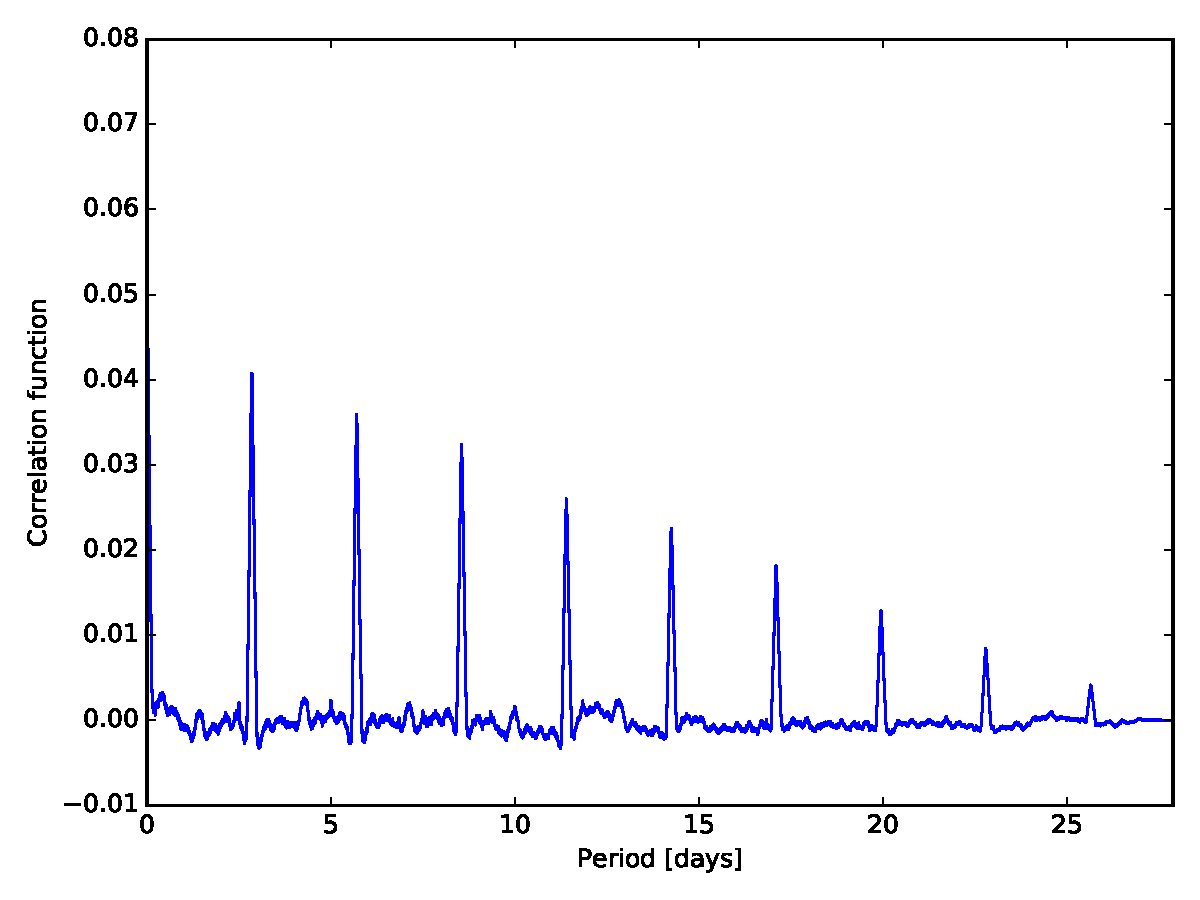
\includegraphics[width=0.9\textwidth]{../figures/2018-11-19_14:46:56_correlation_fig0.pdf}
\end{frame}

\begin{frame}
\frametitle{Autocorrelation + Peaks + Gaussian}
\centering
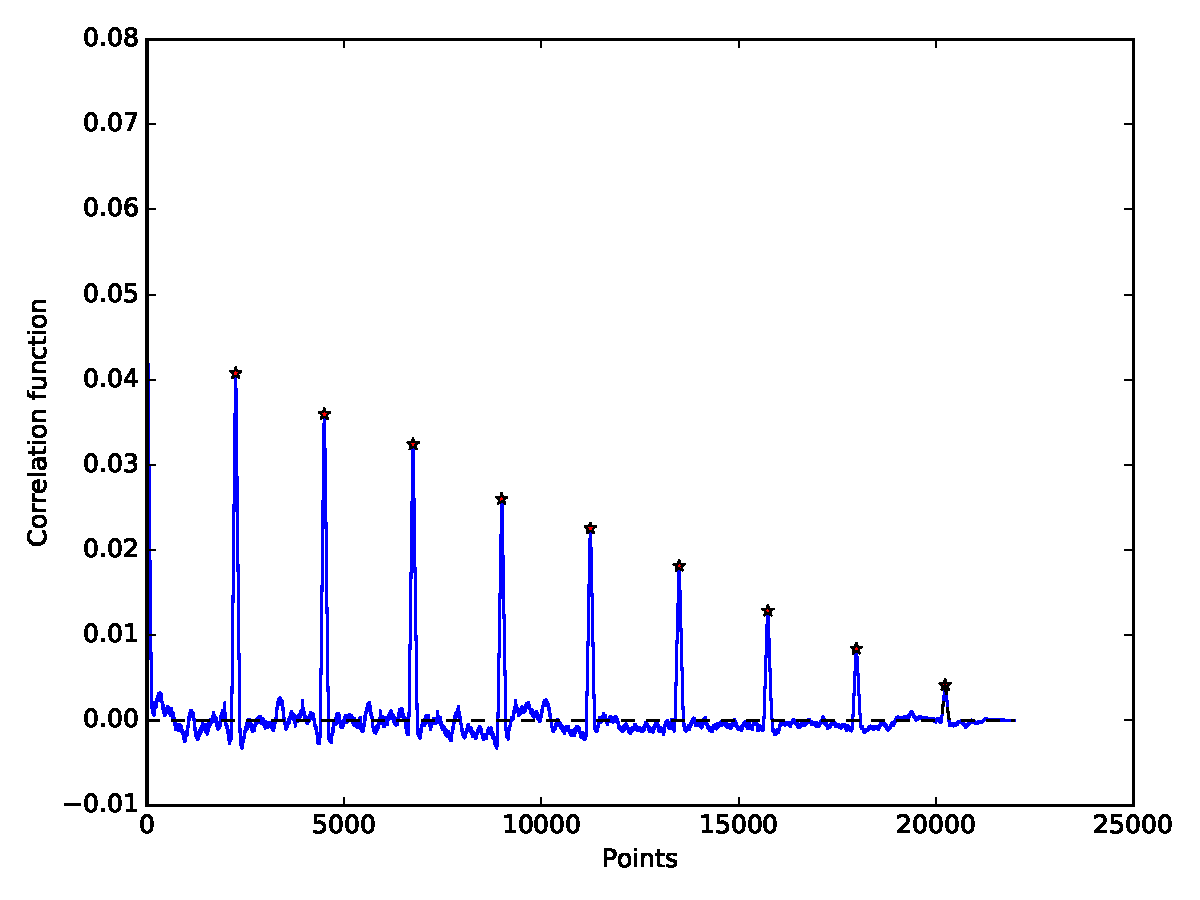
\includegraphics[width=0.9\textwidth]{../figures/2018-11-20_11:12:6_peaks_fig0.pdf}
\end{frame}

\begin{frame}
\frametitle{Folded Light Curve}
\centering
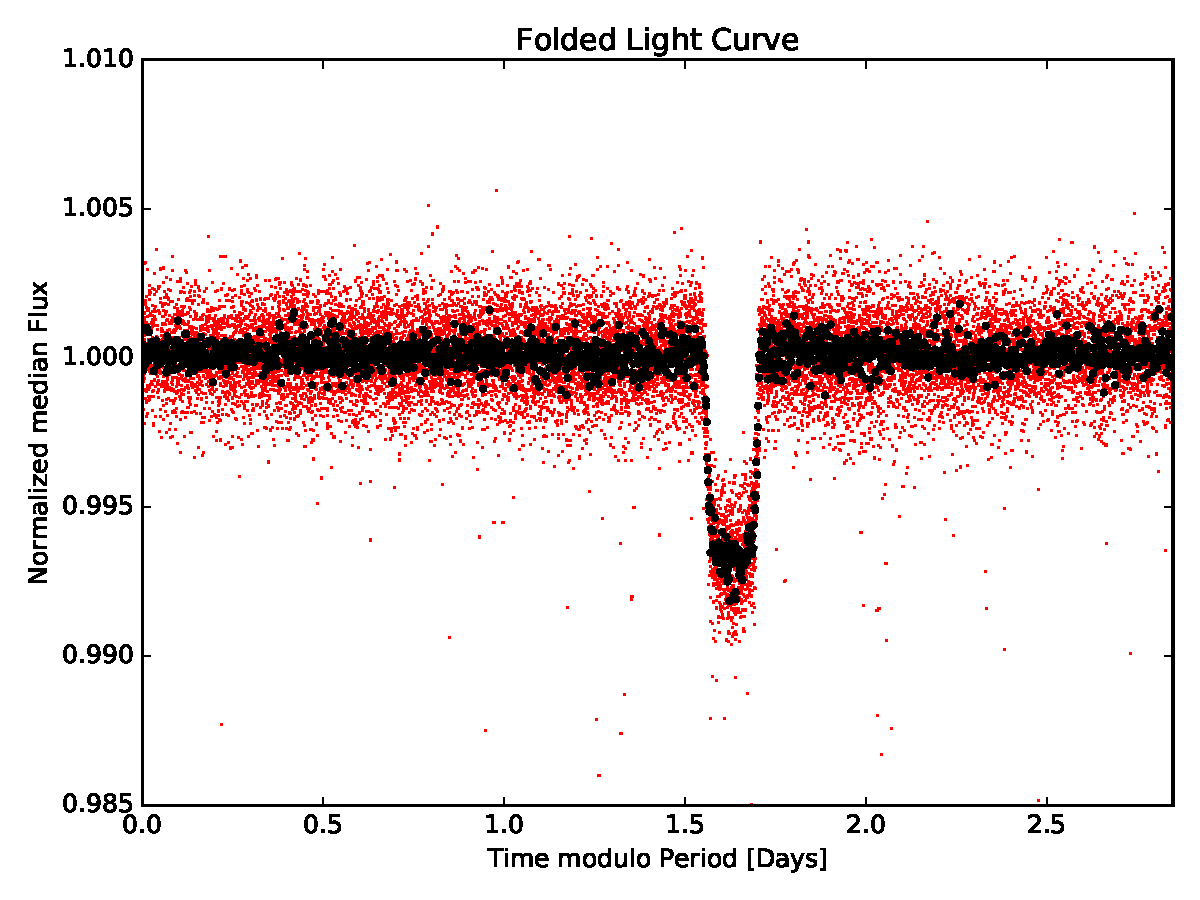
\includegraphics[width=0.9\textwidth]{../figures/2018-11-27_12:41:56_Folded0.pdf}
\end{frame}

\begin{frame}
\frametitle{Fine-mesh Moving Median Filter}
\centering
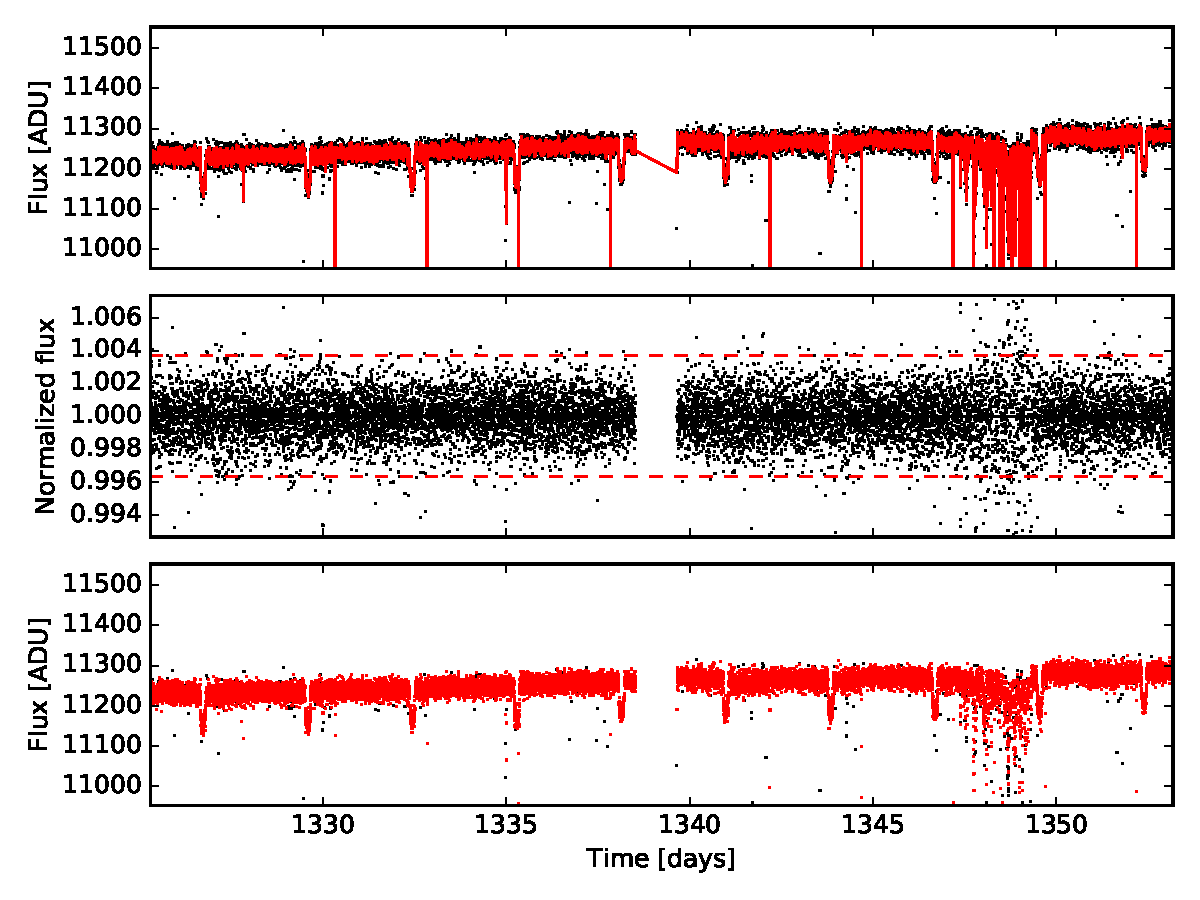
\includegraphics[width=0.9\textwidth]{../figures/2018-11-27_14:45:48_fine_mesh0.pdf}
\end{frame}

\begin{frame}
\frametitle{Fine-mesh Moving Median Filter}
\centering
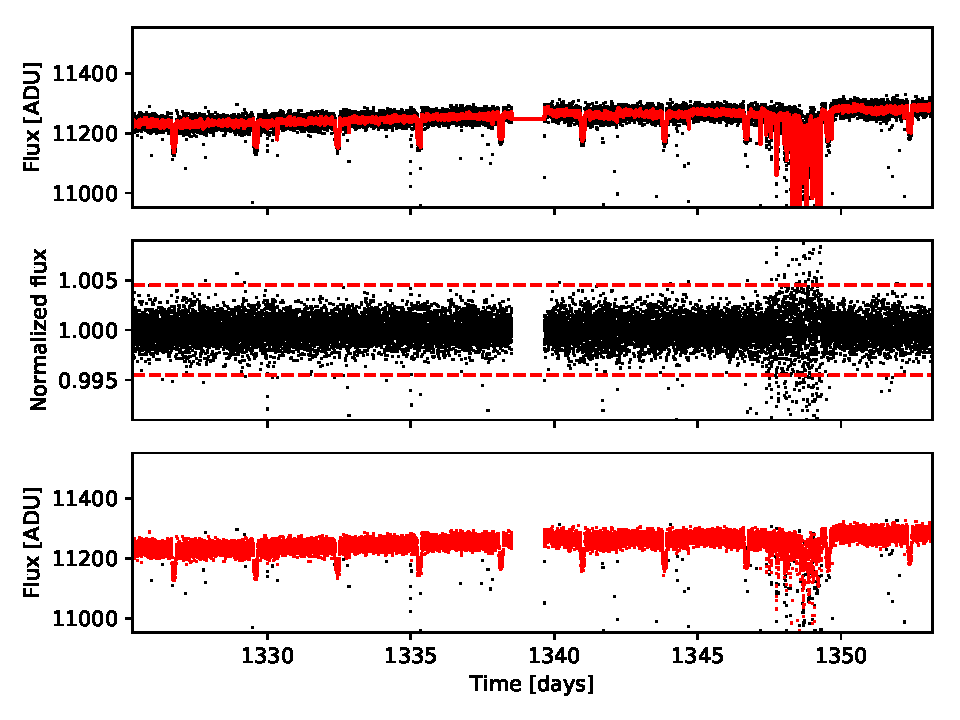
\includegraphics[width=0.9\textwidth]{../figures/2019-1-15_11:5:15_finemesh_TIC38846515.pdf}
\end{frame}

\begin{frame}
\frametitle{Normalization}
\centering
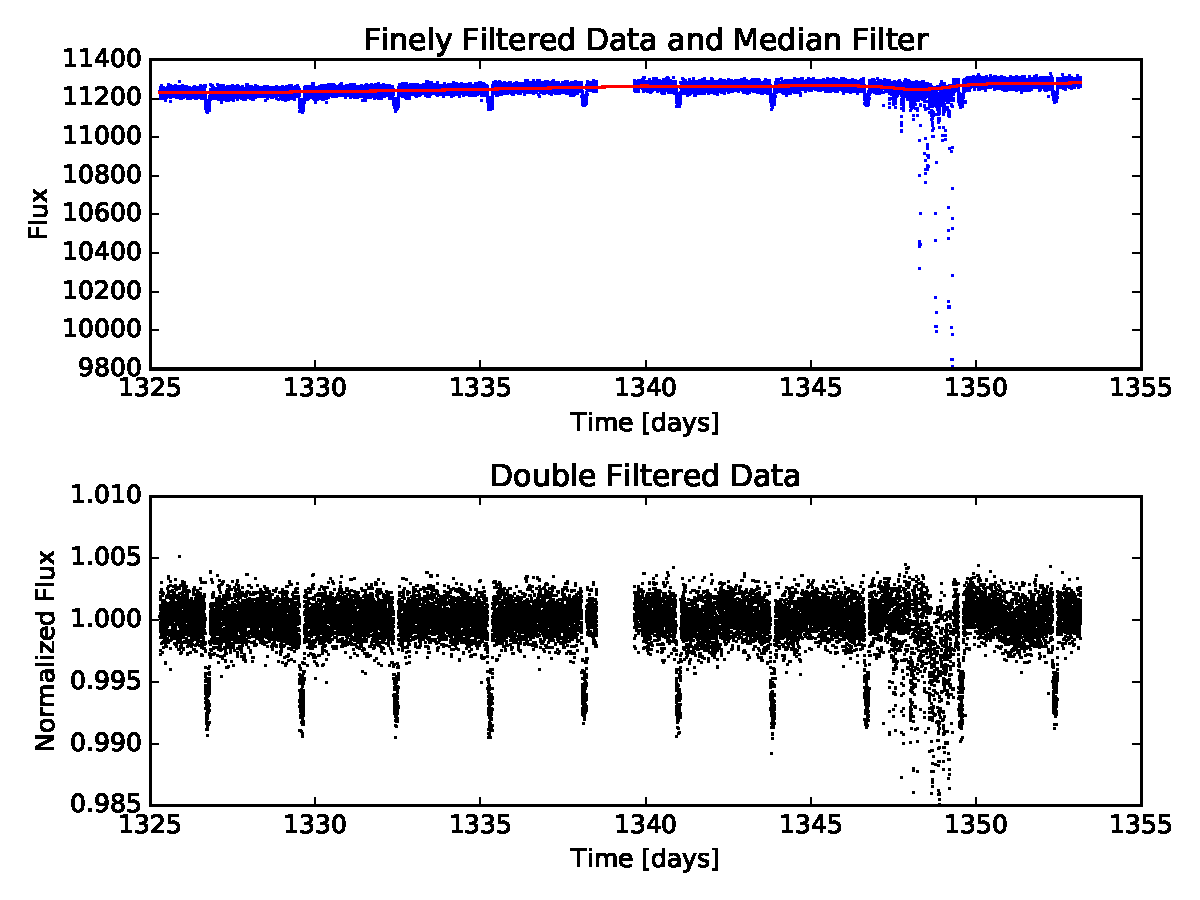
\includegraphics[width=0.9\textwidth]{../figures/2019-1-15_16:2:14_normcurve_lightcurve_TIC38846515.pdf}
\end{frame}

\begin{frame}
\frametitle{if $y[i]>1: y=1$}
\centering
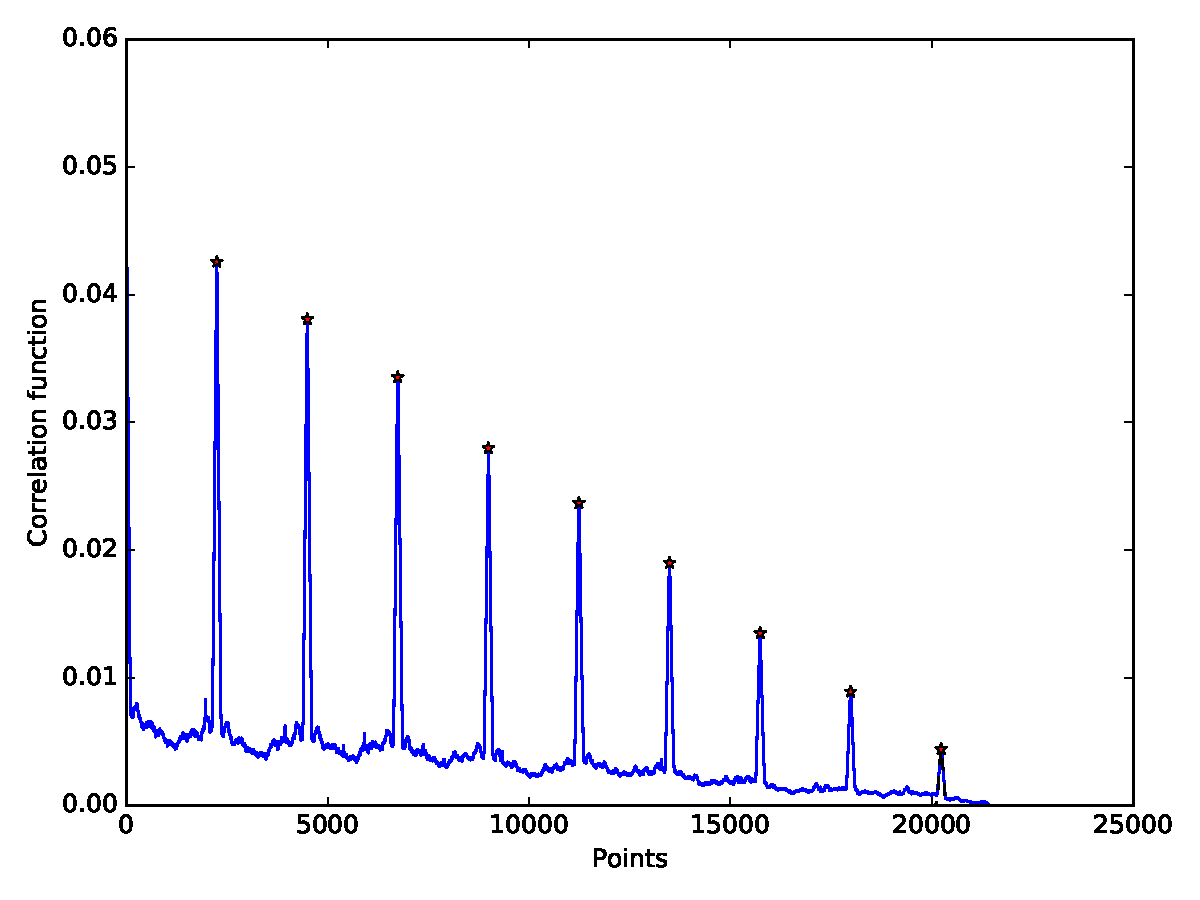
\includegraphics[width=0.9\textwidth]{../figures/2018-11-27_14:45:48_peaks_fig0.pdf}
\end{frame}

\begin{frame}
\frametitle{Interpolation Improvement}
\centering
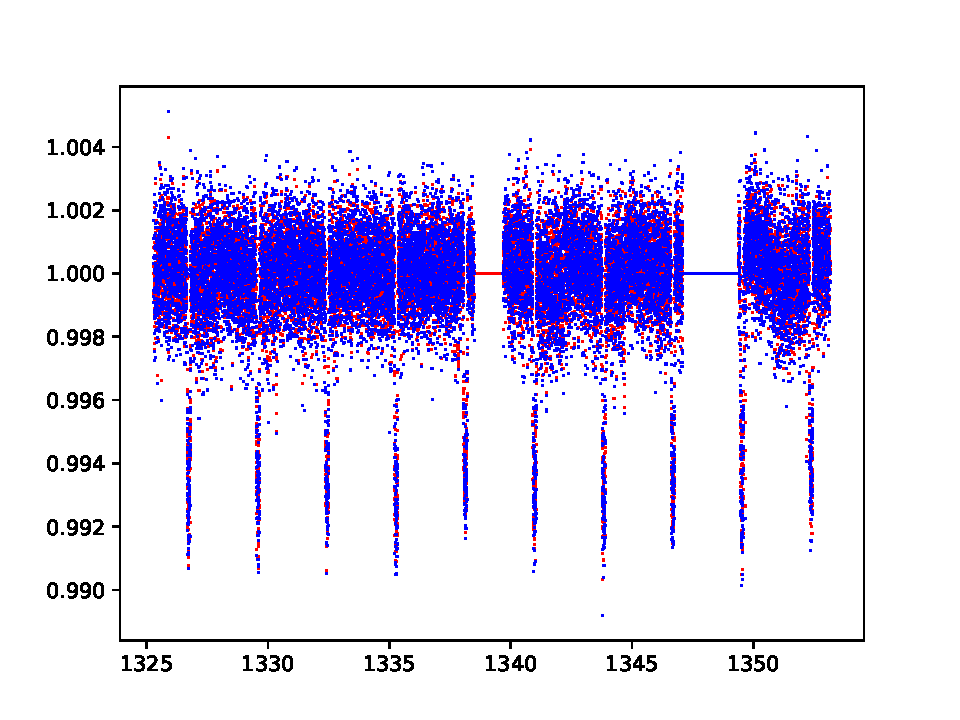
\includegraphics[width=0.9\textwidth]{../figures/2019-1-15_11:5:15_intercurve_TIC38846515.pdf}
\end{frame}

\begin{frame}
\frametitle{Normalized Correlation}
\centering
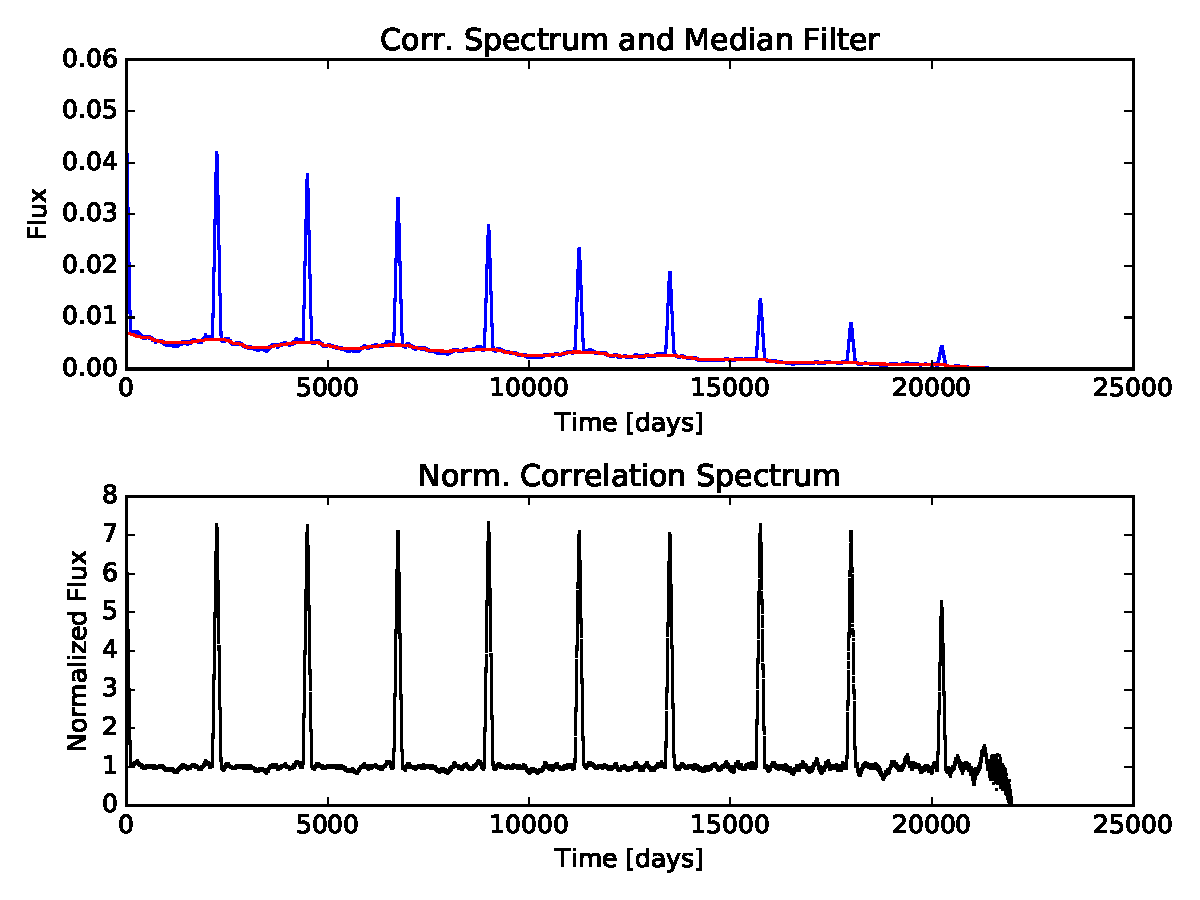
\includegraphics[width=0.9\textwidth]{../figures/2019-1-15_16:2:14_normcurve_correlation_TIC38846515.pdf}
\end{frame}

\begin{frame}
\frametitle{Fitting to All Peaks}
\centering
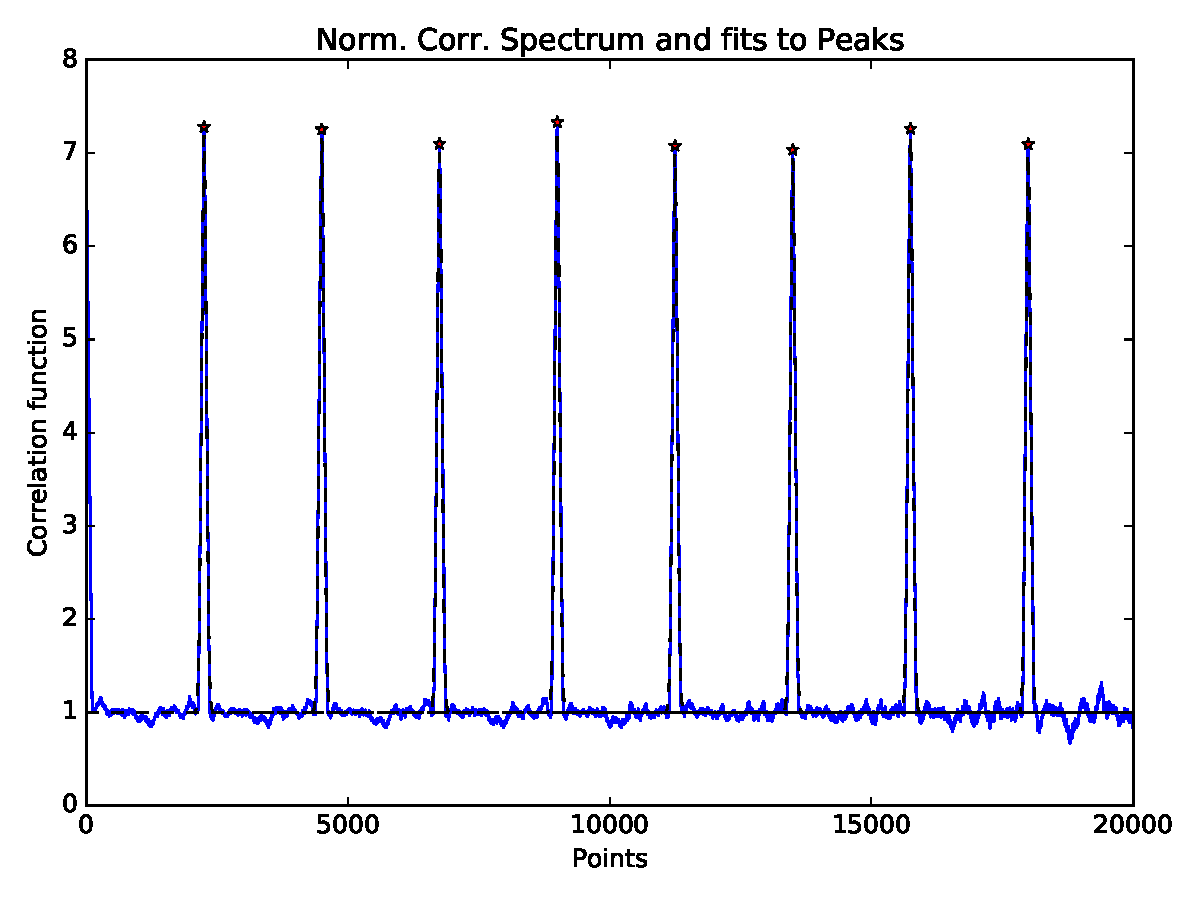
\includegraphics[width=0.9\textwidth]{../figures/2019-1-15_16:2:14_peaks_TIC38846515.pdf}
\end{frame}

\begin{frame}
\frametitle{Linear Fit to Period}
\centering
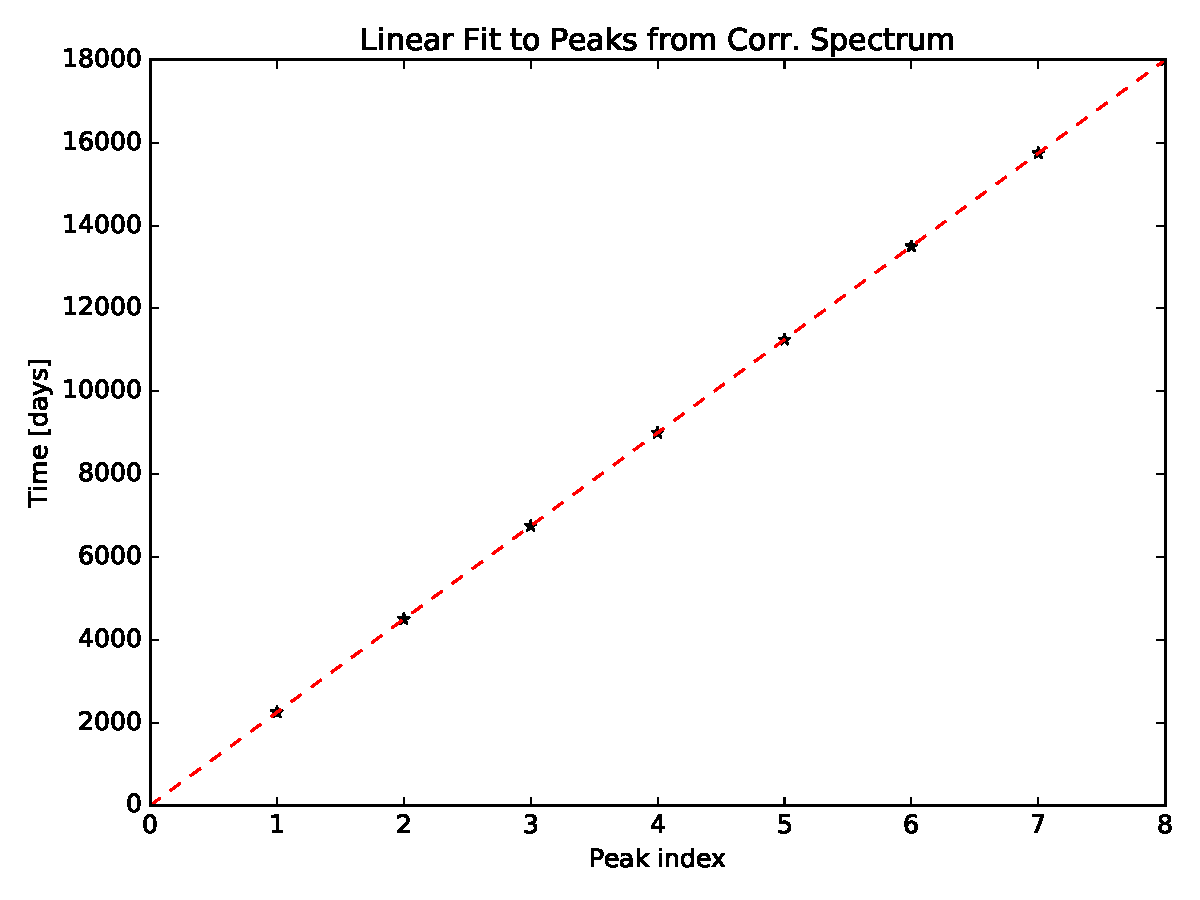
\includegraphics[width=0.9\textwidth]{../figures/2019-1-15_16:2:14_linear_fit_TIC38846515.pdf}
\end{frame}

\begin{frame}
\frametitle{TIC 38846515: Folded Light Curve}
\centering
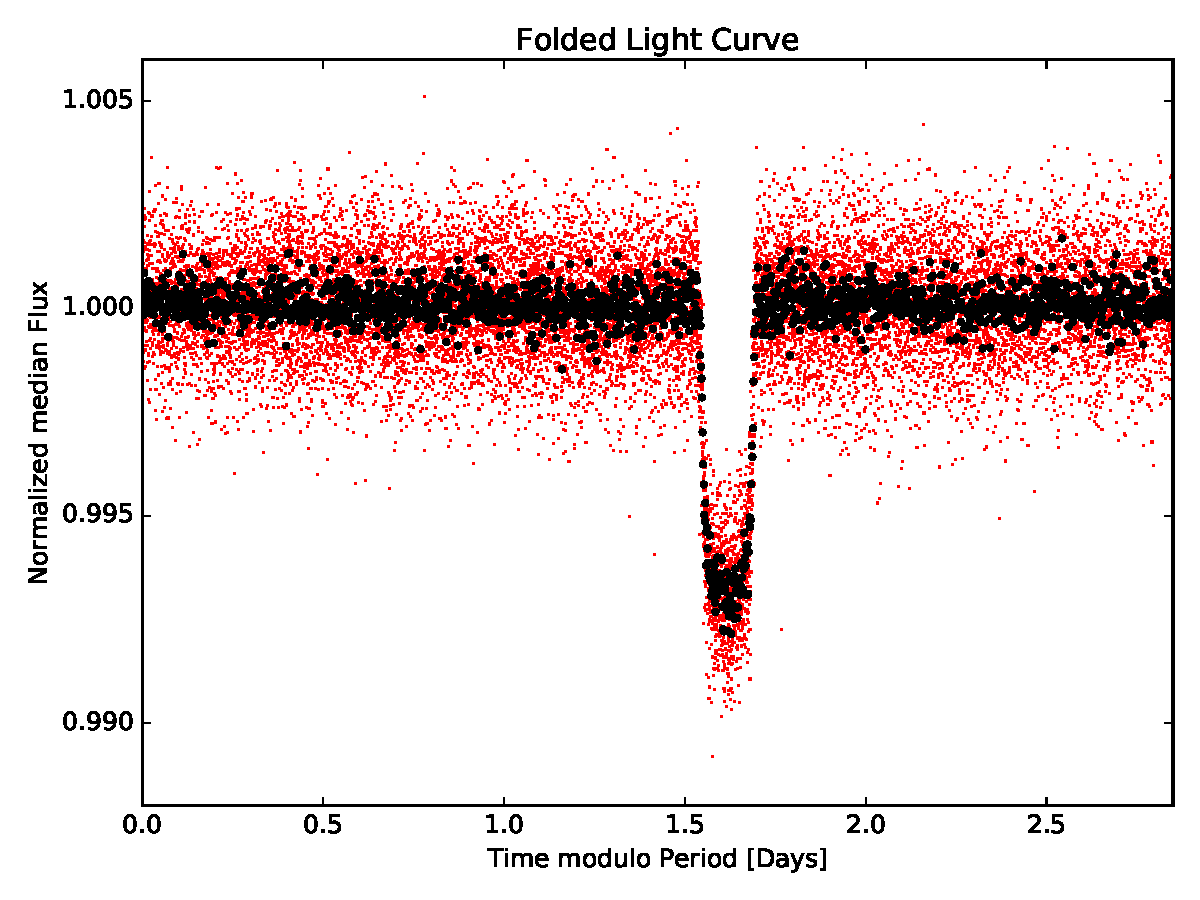
\includegraphics[width=0.9\textwidth]{../figures/2019-1-15_16:2:14_Folded_TIC38846515.pdf}
\end{frame}

\begin{frame}
\frametitle{TIC 76989773: Folded Light Curve}
\centering
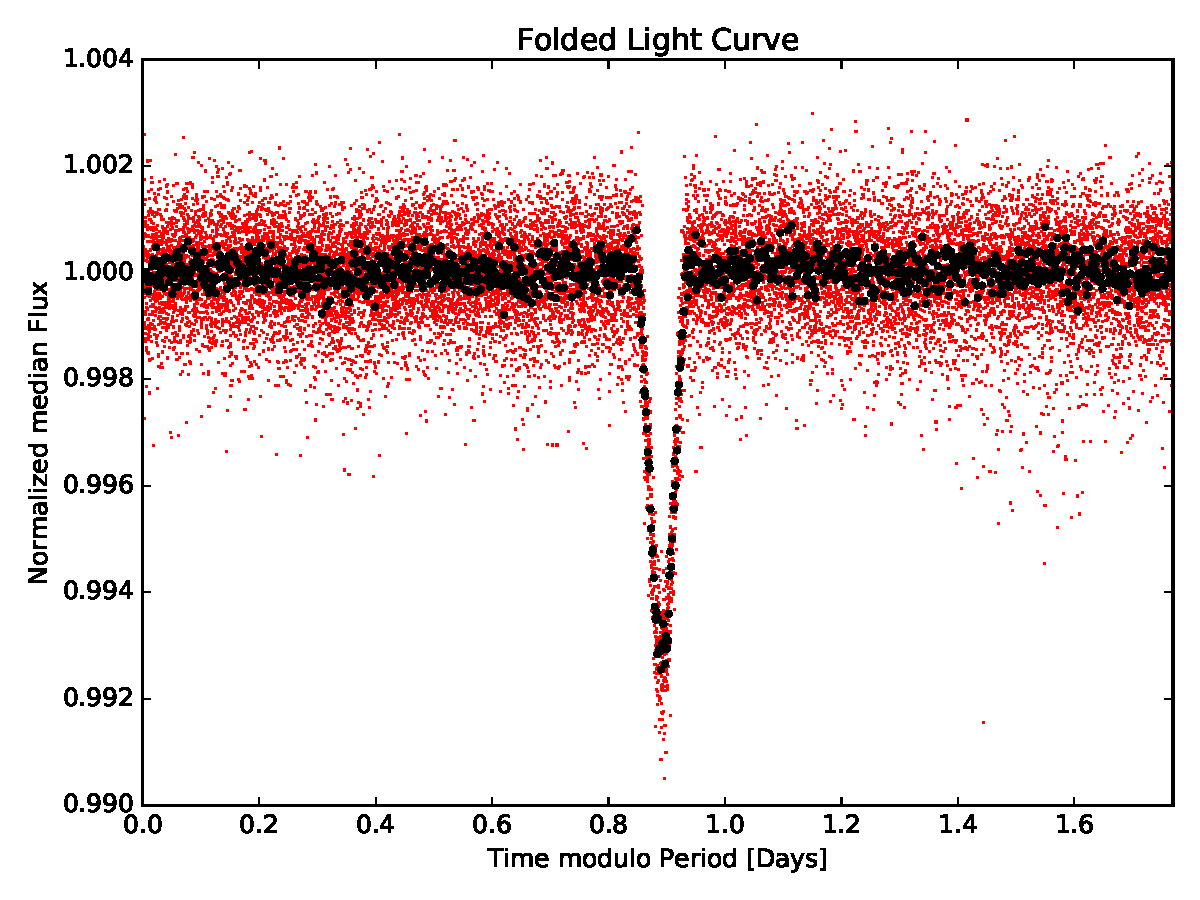
\includegraphics[width=0.9\textwidth]{../figures/2019-1-15_16:2:14_Folded_TIC76989773.pdf}
\end{frame}

\begin{frame}
\frametitle{TIC 201248411: Folded Light Curve}
\centering
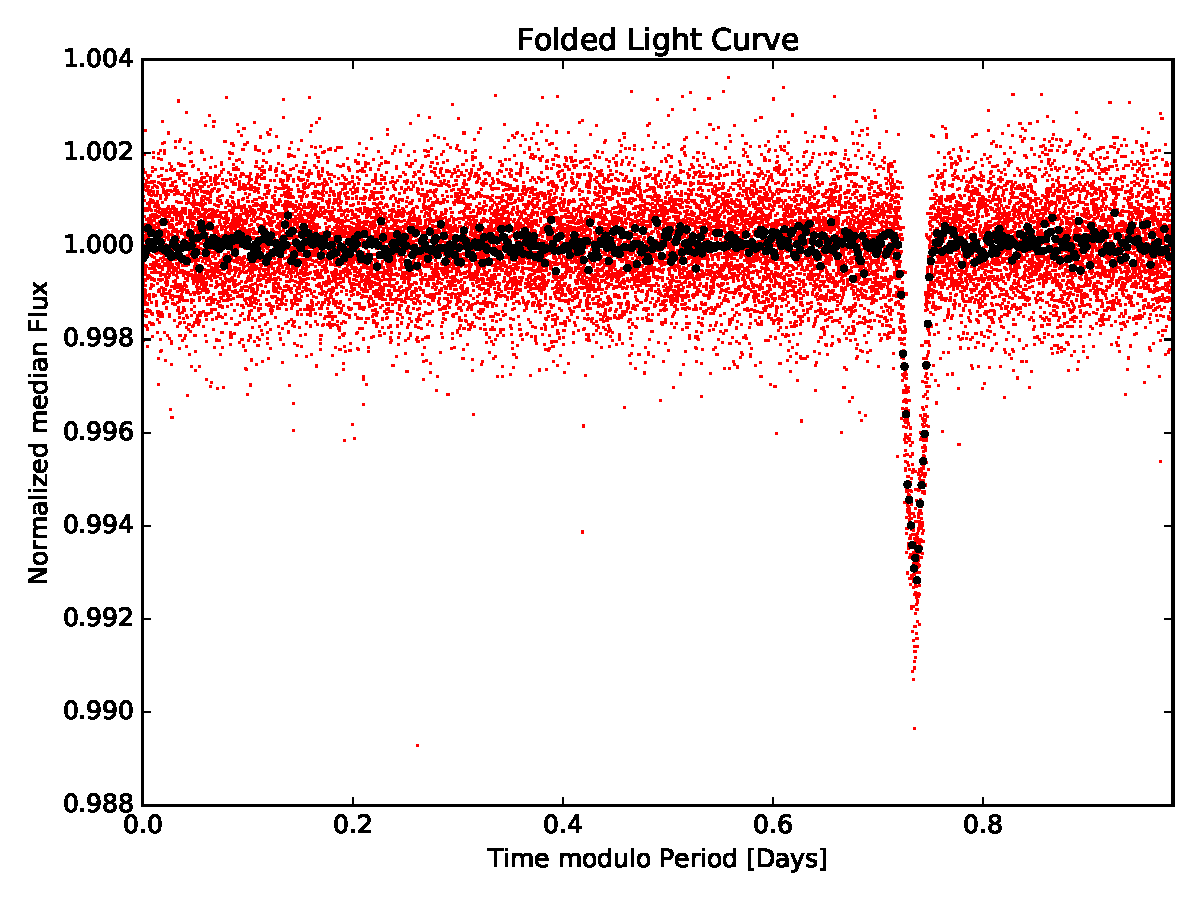
\includegraphics[width=0.9\textwidth]{../figures/2019-1-15_16:2:14_Folded_TIC201248411.pdf}
\end{frame}

\end{document}